\section{Camera Calibration}
A homography can be defined as a tranformation from a projective space onto
itself. As such, it is insufficient when trying to transform objects from a
three-dimensional space to a two-dimensional space, e.g. a cube onto an image
plane. To properly display our cube in the image plane, a projectivty from our
world coordinate system to the image plane is needed. The process of finding
this projectivty is commonly referred to as \emph{camera calibration}
\begin{figure}[htbp]
	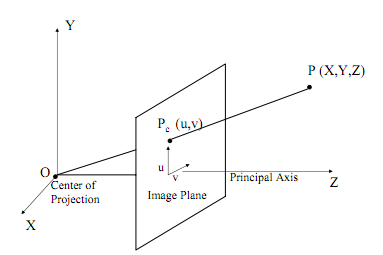
\includegraphics{pics/cameraCalibration.png}
	\caption{Visualization of world-coordinate \emph{(X,Y,Z)}, projection on
	to the image plane. \emph{O} corresponds to the focal point of the
	camera.}
	\label{fig:calibtheory}
\end{figure}

For this assignment, two different methods for calibrating the camera
was utilised:

The first method is that of OpenCV's cameraCalibrate function. By introducing an
object of known dimensions, the camera's parameters can be inferred. The focal
length('s) can be found by the formula $$fx = \frac{dx}{dX} * dZ,\quad fy =
\frac{dy}{dY} * dZ$$ Where $fx$ and $fy$ are the focal length expressed in
pixels on the $x$ and $y$ axes of the image respectively.

